% -----------------------------------------------------------------------
%  lifelines-hc -- SoftwareX Original Software Publication
%
%  Structure follows the SoftwareX required section order:
%    Code metadata table | Motivation and significance | Software description
%    | Illustrative examples | Impact | Conclusions
%
%  NOTE ON CLASS: built here with `article` because elsarticle is not
%  installable in the build environment. At submission, paste the body into
%  Elsevier's SoftwareX Overleaf template (elsarticle + the official
%  metadata table macros). No content changes are needed.
%
%  Compile: pdflatex main && bibtex main && pdflatex main && pdflatex main
% -----------------------------------------------------------------------
\documentclass[11pt]{article}

\usepackage[margin=1in]{geometry}
\usepackage{microtype}
\usepackage{booktabs}
\usepackage{graphicx}
\usepackage{amsmath}
\usepackage{array}
\usepackage{float}
\usepackage{natbib}
\usepackage{hyperref}
\usepackage{listings}
\usepackage{xcolor}

\hypersetup{colorlinks=true, linkcolor=blue!60!black,
            citecolor=blue!60!black, urlcolor=blue!60!black}

\lstset{%
  language=Python, basicstyle=\ttfamily\small,
  keywordstyle=\color{blue!65!black}\bfseries,
  commentstyle=\color{gray!70}, stringstyle=\color{green!45!black},
  breaklines=true, frame=tb, framesep=4pt,
  backgroundcolor=\color{gray!7}, xleftmargin=1.2em, xrightmargin=1.2em,
  aboveskip=0.8em, belowskip=0.5em, showstringspaces=false,
}

\graphicspath{{./}{../figs/}}

\newcolumntype{L}[1]{>{\raggedright\arraybackslash}p{#1}}

\title{\texttt{lifelines-hc}: Higher Criticism testing for sparse
  non-proportional hazard departures in Python}

\author{%
  Alon Kipnis\thanks{School of Computer Science, Reichman University,
    Herzliya 4610101, Israel. Corresponding author:
    \href{mailto:alon.kipnis@runi.ac.il}{alon.kipnis@runi.ac.il}}
  \and
  Ben Galili\thanks{Department of Computer Science, Technion -- Israel
    Institute of Technology, Haifa 3200003, Israel}
  \and
  Zohar Yakhini\thanks{School of Computer Science, Reichman University,
    Herzliya 4610101, Israel; and Department of Computer Science,
    Technion -- Israel Institute of Technology, Haifa 3200003, Israel}%
}
\date{}

\begin{document}
\maketitle

\begin{abstract}
The log-rank test is the standard tool for two-sample survival comparison,
but it loses power when the hazard difference is confined to a small,
unknown subset of the follow-up. Weighted log-rank tests each fix a
temporal emphasis in advance; combination procedures such as MaxCombo and
the Yang--Prentice short-term/long-term hazard-ratio model scan a small
dictionary of global temporal shapes. All remain insensitive to \emph{sparse}
departures falling outside those shapes. We present \texttt{lifelines-hc},
a Python package that extends the \texttt{lifelines} survival library with
the HCHG test of \citet{kipnis_biometrika}: Higher Criticism applied to
per-interval hypergeometric $p$-values. The package exposes a
\texttt{lifelines}-compatible API, returns interval-level diagnostics
identifying which time windows drive a detection, and ships a benchmarking
wrapper that runs HCHG alongside the log-rank test, four weighted
alternatives, MaxCombo and Yang--Prentice in one call. On four clinical
datasets with distinct non-proportional structures, HCHG attains
$p \leq 0.014$ throughout where the log-rank test is non-significant
everywhere ($p \geq 0.26$), and detects the three departures that MaxCombo
and Yang--Prentice miss.
\end{abstract}

\noindent\textbf{Keywords:} survival analysis; higher criticism; sparse
signal detection; non-proportional hazards; hypergeometric test; Python.

\vspace{1em}

% =======================================================================
\section*{Code metadata}
% =======================================================================

\begin{table}[H]
\centering
\small
\begin{tabular}{@{}lL{4.2cm}L{7.4cm}@{}}
\toprule
\textbf{Nr.} & \textbf{Code metadata description} & \textbf{Value} \\
\midrule
C1 & Current code version & v0.1.2 \\[2pt]
C2 & Permanent link to code/repository used for this code version &
     \url{https://github.com/alonkipnis/lifelines-hc/tree/v0.1.2} \\[2pt]
C3 & Permanent link to archived version &
     \url{https://doi.org/10.5281/zenodo.23170282} \\[2pt]
C4 & Legal code license & MIT \\[2pt]
C5 & Code versioning system used & git \\[2pt]
C6 & Software code languages, tools and services used &
     Python; R (optional, only for the MaxCombo and Yang--Prentice
     comparators) \\[2pt]
C7 & Compilation requirements, operating environments, dependencies &
     Python $\geq$ 3.8; \texttt{numpy}, \texttt{pandas},
     \texttt{lifelines} $\geq$ 0.29, \texttt{multiple-hypothesis-testing},
     \texttt{multiHGtest}. Optional: \texttt{matplotlib} for plotting;
     R with \texttt{nph} and \texttt{YPmodel} for the comparator tests.
     Platform independent. \\[2pt]
C8 & Link to developer documentation/manual &
     \url{https://github.com/alonkipnis/lifelines-hc/blob/v0.1.2/README.md} \\[2pt]
C9 & Support email for questions &
     \href{mailto:alon.kipnis@runi.ac.il}{alon.kipnis@runi.ac.il} \\
\bottomrule
\end{tabular}
\caption{Code metadata.}
\label{tab:codemeta}
\end{table}

% =======================================================================
\section{Motivation and significance}
% =======================================================================

The Kaplan--Meier estimator \citep{kaplan1958} and the log-rank test
\citep{mantel1966} are the workhorses of two-sample survival analysis.
The log-rank statistic has good power against proportional-hazards
alternatives \citep{schoenfeld1981}, and this is the regime for which it
was designed. \citet{kipnis_biometrika} showed that it is not optimal
against \emph{sparse} hazard departures, in which the hazard difference is
concentrated in a small, unknown subset of time intervals.

Such departures are common in contemporary trials. Immune checkpoint
inhibitors may require an immune-priming phase before producing durable
tumour suppression, giving delayed effects and crossing curves: in
CheckMate~057, nivolumab improved overall survival relative to docetaxel
while the progression-free survival curves crossed \citep{borghaei2015}.
Targeted therapies can produce benefits confined to a limited window that
are diluted in global summaries: in COMET-1, cabozantinib markedly improved
bone scan response at week~12 and radiographic progression-free survival
without a significant overall survival benefit \citep{smith2016}.
Subgroup-dependent biology generates composite, time-varying differences:
in AZURE, adjuvant zoledronic acid showed no overall benefit but did
benefit women with established menopause \citep{coleman2011,coleman2014}.
Time-varying treatment effects can produce multi-window departures: in the
CSL cirrhosis trial, prednisone was harmful early and beneficial later,
yielding curves that cross more than once \citep{csl_data}.

Several weighted log-rank tests address non-proportional hazards
\citep{gehan1965,peto1972,taroneware1977,harrington1982,flemingharrington1991}.
Each applies a temporal weight emphasising early, intermediate or late
events, and each has good power when the signal matches its intended
pattern --- but choosing the weight requires knowing in advance
\emph{where} the departure will occur. Contemporary practice therefore
combines several weights rather than committing to one. MaxCombo
\citep{lin2020maxcombo,ristl2021nph} takes the maximum of
$\mathrm{FH}(\rho,\gamma)$ statistics over
$(\rho,\gamma)\in\{(0,0),(0,1),(1,0),(1,1)\}$ with a multiplicity-adjusted
$p$-value; the Yang--Prentice model \citep{yang2005} interpolates between
an immediate hazard ratio $\theta_1$ and an asymptotic ratio $\theta_2$,
with an associated adaptive weighted log-rank test \citep{yang2010improved}.
Both are powerful against the global early-versus-late patterns they were
designed for. Both remain averaging methods over a small dictionary of
global temporal shapes, and can miss sparse or multi-window departures.

No implementation of a scan-based alternative was available to Python users
of \texttt{lifelines} \citep{davidsonpilon2019}, the most widely used
survival library in that ecosystem. \texttt{lifelines-hc} fills that gap:
it implements HCHG \citep{kipnis_biometrika}, requires no a priori temporal
weight, and reports which intervals drive a detection --- information that
no single-number test provides.

% =======================================================================
\section{Software description}
% =======================================================================

\subsection{Software architecture}

\texttt{lifelines-hc} is a pure-Python package of two modules.
\texttt{lifelines\_hc.statistics} implements the interval construction, the
exact hypergeometric per-interval $p$-values, the Higher Criticism
aggregation, and the permutation calibration;
\texttt{lifelines\_hc.plotting} provides Kaplan--Meier overlays and
$p$-value profile plots. Every test returns a
\texttt{lifelines.statistics.StatisticalResult}, the same object returned by
\texttt{lifelines.statistics.logrank\_test}, so results drop into existing
\texttt{lifelines} workflows and print with the library's own summary
formatting. The package adds no state and subclasses nothing; it is a set of
functions over NumPy arrays.

Given two groups with right-censored observations $(T_i, E_i, G_i)$, the
follow-up range is partitioned into $K$ equal-width intervals. For interval
$k$, let $n_k$ be the total events, $r_k^A, r_k^B$ the subjects at risk in
each group, and $x_k$ the events in group~B. Under the null of equal
group-specific hazards,
%
\begin{equation}\label{eq:hypergeom}
  x_k \;\big|\; n_k, r_k^A, r_k^B
  \;\sim\; \mathrm{Hypergeometric}\!\left(r_k^A + r_k^B,\; r_k^B,\; n_k\right),
\end{equation}
%
yielding an exact one-sided $p$-value $p_k$ per interval. Ordering these as
$p_{(1)} \leq \cdots \leq p_{(K)}$, the HC statistic
\citep{donoho2004,donoho2015special} is
%
\begin{equation}\label{eq:hc}
  \mathrm{HCHG}_K \;=\;
  \max_{1 \leq j \leq \lfloor\gamma K\rfloor}
  \frac{j/K - p_{(j)}}{\sqrt{p_{(j)}\left(1 - p_{(j)}\right)/K}},
\end{equation}
%
where $\gamma \in (0,1)$ (default $0.2$) restricts the scan to the most
extreme fraction of interval $p$-values. A global $p$-value follows from
permuting group labels. For the two-sided alternative, the minimum of the
two one-sided interval $p$-values replaces $p_k$ in~(\ref{eq:hc}).

Interval pooling is the one parameter requiring user attention. With
continuous event times each distinct time carries at most one event, and the
hypergeometric $p$-values are then too coarse to be informative; pooling
events into $K$ equal-width intervals via \texttt{n\_intervals\_to\_pool}
restores resolution. Values between 50 and 200 work well in practice, and
the parameter may be omitted for naturally discrete or heavily tied data.

\subsection{Software functionalities}

\begin{itemize}\itemsep2pt
\item \texttt{higher\_criticism\_test} --- the HCHG test, with exact
      permutation calibration, one- or two-sided alternatives, optional
      censoring indicators, and a configurable HC fraction $\gamma$.
\item \texttt{berk\_jones\_test}, \texttt{fisher\_combination\_test},
      \texttt{min\_p\_test} --- alternative aggregations of the same
      per-interval $p$-values, for sensitivity analysis.
\item \texttt{event\_pvalues} --- the raw per-interval $p$-values.
\item \texttt{suspected\_deviations} --- a \texttt{pandas.DataFrame} of
      per-interval $p$-values with a boolean \texttt{suspected} column
      marking intervals at or below the HC threshold. This is the
      diagnostic output distinguishing HCHG from a single-number test: it
      localises the departure.
\item \texttt{plot\_km\_with\_hc}, \texttt{plot\_pvalue\_profile} ---
      Kaplan--Meier curves with flagged intervals shaded, and signed
      $-\log_{10}$ $p$-value profiles.
\item \texttt{run\_all\_tests} --- a benchmarking wrapper returning a
      \texttt{DataFrame} comparing HCHG, log-rank, Gehan--Wilcoxon,
      Tarone--Ware, Peto--Prentice, Fleming--Harrington$(1,1)$, MaxCombo and
      the Yang--Prentice adaptive log-rank test on one dataset.
\end{itemize}

\begin{lstlisting}
from lifelines_hc import higher_criticism_test, suspected_deviations

result = higher_criticism_test(
    T_A, T_B,
    event_observed_A=E_A, event_observed_B=E_B,
    n_intervals_to_pool=100, n_permutations=2000,
    alternative='both', gamma=0.2, seed=42)

print(result.p_value)         # permutation-calibrated p-value
print(result.test_statistic)  # HCHG statistic

flagged = suspected_deviations(T_A, T_B, n_intervals_to_pool=100)
print(flagged[flagged["suspected"]])   # which windows drive the signal
\end{lstlisting}

% =======================================================================
\section{Illustrative examples}
% =======================================================================

We apply \texttt{lifelines-hc} to four clinical datasets with distinct
non-proportional structures (Figure~\ref{fig:main}), benchmarking HCHG
against the log-rank test, four weighted alternatives, MaxCombo and
Yang--Prentice. Throughout, HCHG uses two-sided interval $p$-values,
$\gamma = 0.2$, and 2000 label permutations with the seed fixed at 42.
Individual patient data for the first three trials were reconstructed from
published Kaplan--Meier curves using the algorithm of \citet{guyot2012};
the CSL trial provides public individual patient data.

\begin{figure}[t!]
  \centering
  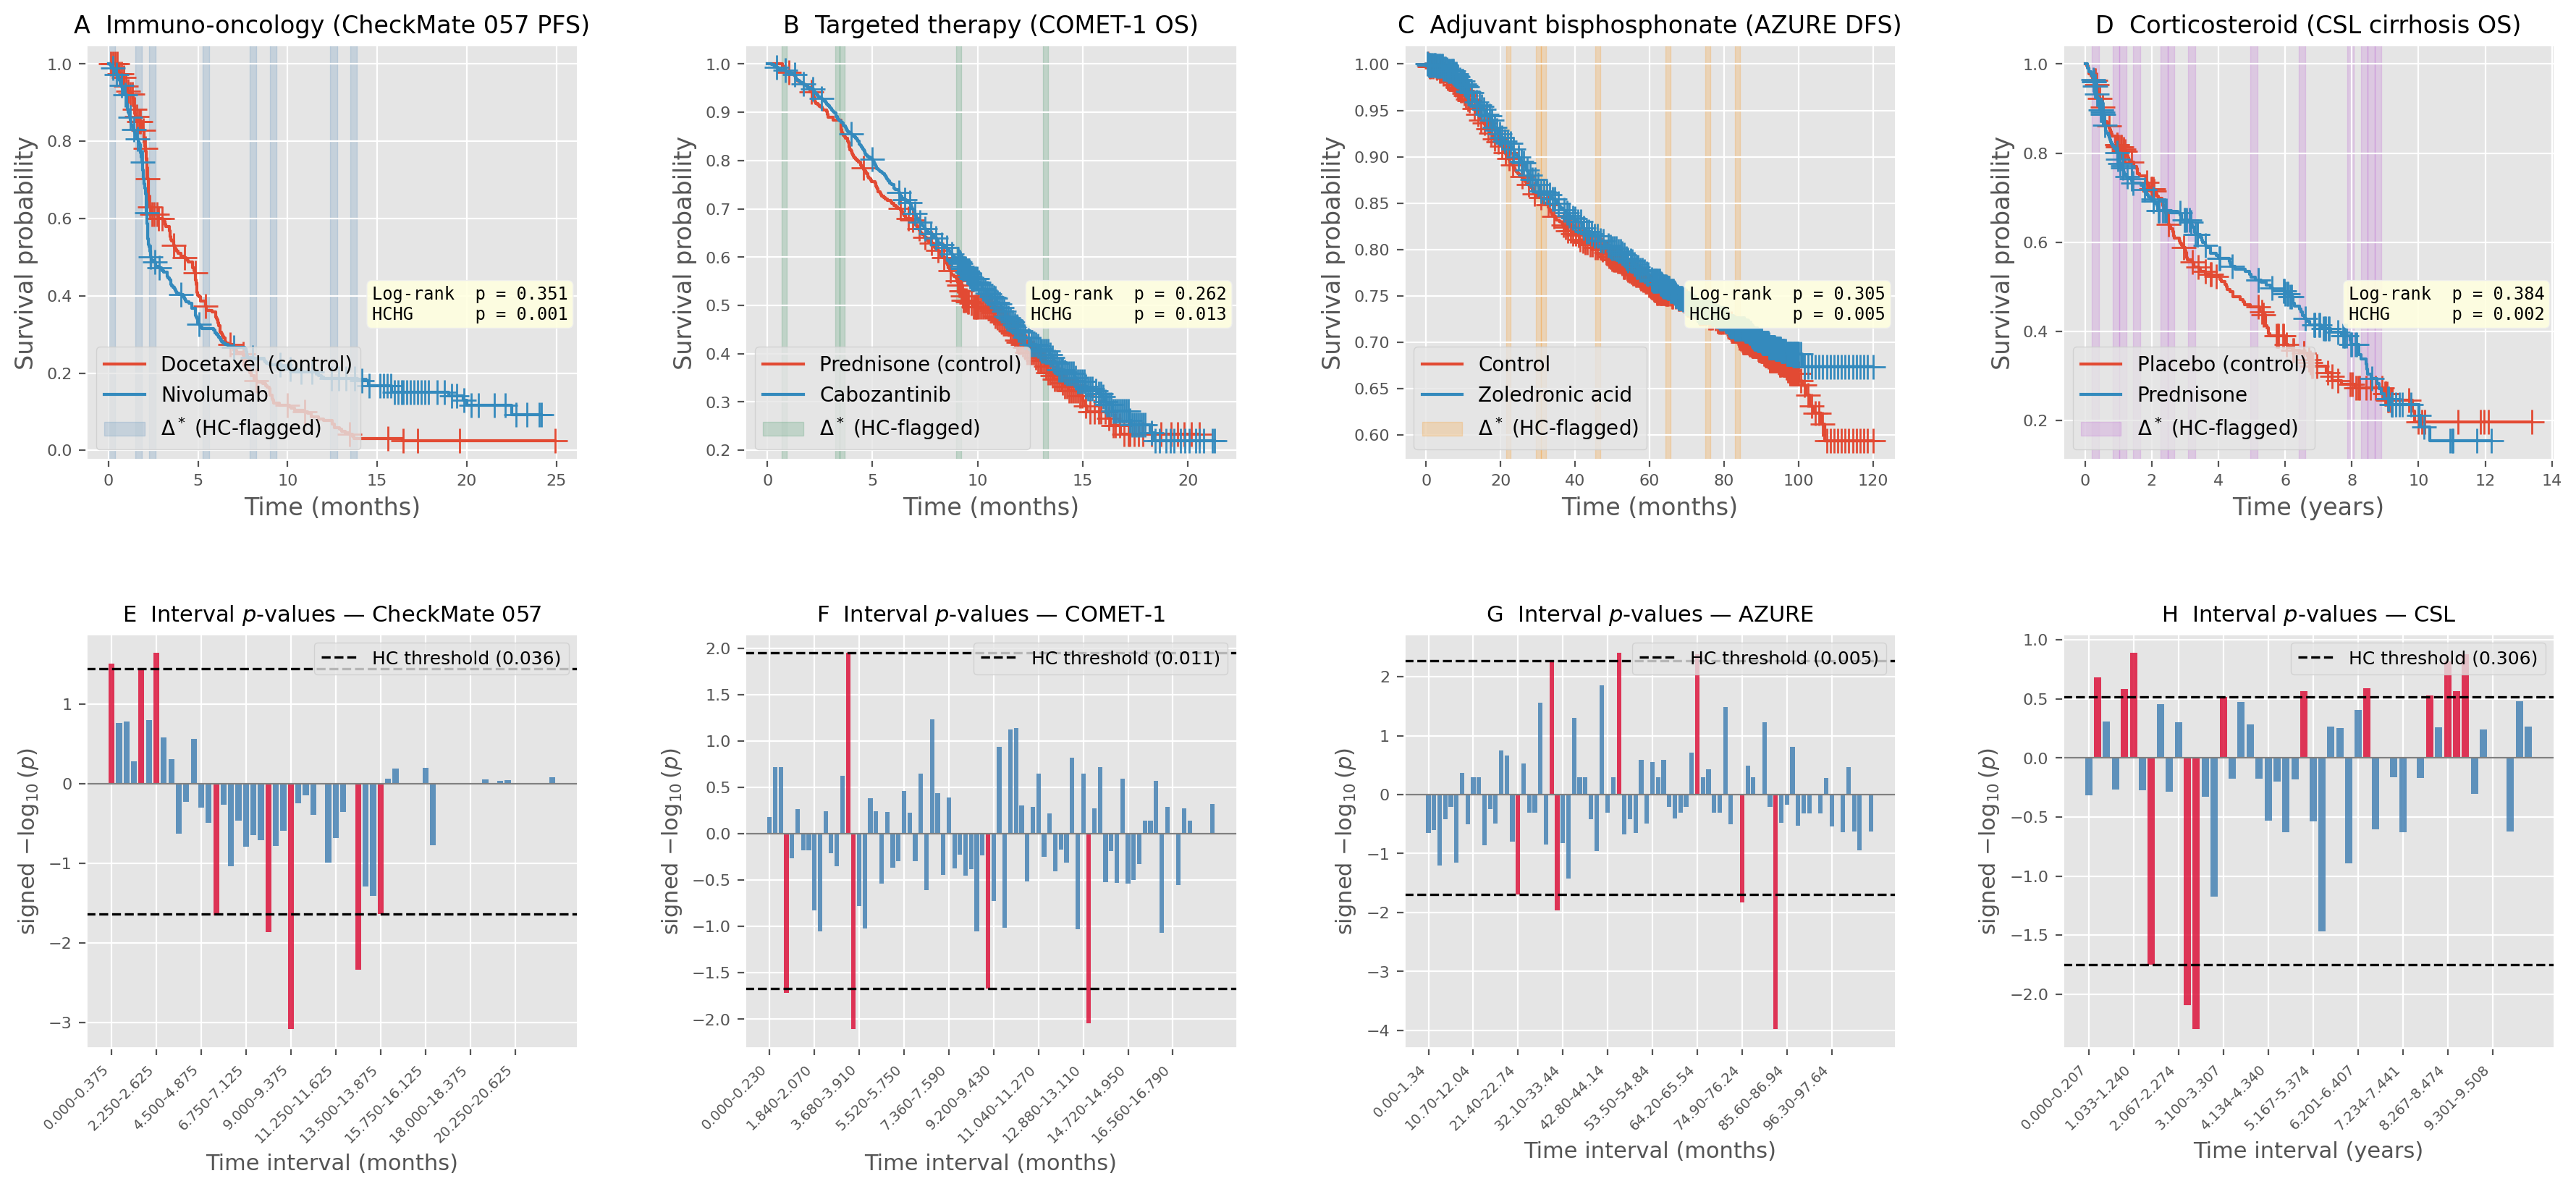
\includegraphics[width=\textwidth]{figure1_4dom}
  \caption{%
    \textbf{Higher Criticism detects non-proportional hazard departures
    across four clinical datasets with distinct temporal patterns.}
    Top row (A--D): Kaplan--Meier curves with HCHG-flagged intervals
    shaded. Bottom row (E--H): per-interval \emph{signed}
    $-\log_{10}$(hypergeometric $p$-value); upward bars mark excess events
    in the treatment arm, downward bars excess in the control arm. Dashed
    lines are the per-direction HCHG thresholds; bars beyond either line
    are highlighted and coincide with the intervals shaded above.
    \textbf{(A,E)}~CheckMate~057 PFS ($n=582$); log-rank $p=0.351$,
    HCHG $p=0.001$.
    \textbf{(B,F)}~COMET-1 OS ($n=1028$); log-rank $p=0.262$,
    HCHG $p=0.014$.
    \textbf{(C,G)}~AZURE DFS ($n=3359$); log-rank $p=0.305$,
    HCHG $p=0.005$.
    \textbf{(D,H)}~CSL OS ($n=446$, fully public raw data);
    log-rank $p=0.384$, HCHG $p=0.002$.%
  }
  \label{fig:main}
\end{figure}

\paragraph{Crossing curves (CheckMate~057).}
582 patients with advanced non-squamous NSCLC randomised to nivolumab
($n=292$) or docetaxel ($n=290$) \citep{borghaei2015}. Progression-free
survival curves cross at $\sim$3 months. The log-rank test is
non-significant ($p = 0.351$) as early excess and late benefit cancel.
Gehan--Wilcoxon ($p = 0.041$) and Peto--Prentice ($p = 0.049$) reach
borderline significance; Tarone--Ware ($p = 0.358$) and
Fleming--Harrington$(1,1)$ ($p = 0.256$) do not. This is the delayed-benefit
pattern MaxCombo and Yang--Prentice target, and both succeed: MaxCombo
$p = 2.5 \times 10^{-5}$, driven by the late-weighted $\mathrm{FH}(0,1)$
member ($Z = 4.27$), and Yang--Prentice $p = 0.00055$ with
$\hat\theta_1 = 2.33$, $\hat\theta_2 = 0.44$. HCHG achieves $p = 0.001$ and
additionally flags both the early divergence and the late separation
windows separately.

\paragraph{Transient early benefit (COMET-1).}
1028 patients with chemotherapy-pretreated mCRPC randomised 2:1 to
cabozantinib ($n=682$) or prednisone ($n=346$) \citep{smith2016}.
Cabozantinib significantly improved bone scan response at week~12 without a
sustained survival benefit, giving a temporally concentrated advantage in
months~3--7. The log-rank test gives $p = 0.262$ and all four weighted
alternatives are non-significant ($p \geq 0.19$). MaxCombo ($p = 0.338$) and
Yang--Prentice ($p = 0.262$) also miss it: a transient few-month advantage
is not a global early-versus-late hazard-ratio shape. HCHG gives
$p = 0.014$, aggregating evidence across the specific early intervals where
the effect is concentrated.

\paragraph{Mid-window accumulation (AZURE).}
3359 early-stage breast cancer patients randomised to standard adjuvant
therapy with ($n=1681$) or without ($n=1678$) zoledronic acid
\citep{coleman2011,coleman2014}. The drug's benefit depends on the
low-oestrogen postmenopausal state; as premenopausal patients transitioned
during the decade-long follow-up, the hazard difference accumulated in
months~20--60 rather than uniformly. Log-rank $p = 0.305$, all weighted
alternatives $p \geq 0.28$, MaxCombo $p = 0.401$, Yang--Prentice
$p = 0.308$. HCHG gives $p = 0.005$. The detection is corroborated by the
published subgroup analyses showing significant benefit in postmenopausal
patients, indicating a genuine biological effect rather than an artefact.

\paragraph{Multi-window, sign-changing effect (CSL).}
446 patients with histologically verified liver cirrhosis randomised to
prednisone ($n=226$) or placebo ($n=220$), with 270 deaths over up to
$\sim$13 years \citep{csl_data}. Unlike the preceding three, the raw
individual patient data are public, via the CRAN \texttt{timereg} package
and the SurvSet repository \citep{survset2022}; this example is therefore
reproducible end to end from public sources. Corticosteroids cause early harm
followed by later anti-inflammatory benefit, and the curves cross more than
once. Log-rank $p = 0.384$; Gehan--Wilcoxon $p = 0.51$, Tarone--Ware
$p = 0.38$, Peto--Prentice $p = 0.45$, Fleming--Harrington$(1,1)$
$p = 0.14$; MaxCombo $p = 0.236$, Yang--Prentice $p = 0.393$. HCHG gives
$p = 0.002$: no single temporal weight, and no two-parameter
short-term/long-term hazard ratio, represents a multi-window sign-changing
departure.

\paragraph{Summary.}
Across the four datasets HCHG attains $p \leq 0.014$ in every case while the
log-rank test is non-significant throughout ($p \geq 0.26$). MaxCombo and
Yang--Prentice are significant only on CheckMate~057, the delayed-benefit
crossing they were designed to detect; on the other three they return
$p \geq 0.24$. HCHG is therefore complementary rather than merely
competitive: it matches the combination procedures on global
early-versus-late non-proportionality and retains power where a small
Fleming--Harrington dictionary cannot reach.

% =======================================================================
\section{Impact}
% =======================================================================

\texttt{lifelines-hc} makes a published but previously unimplemented test
available to the Python survival-analysis community. Before this package,
applying HCHG required reimplementing the interval construction, the exact
hypergeometric calculation and the permutation calibration from the
method paper --- enough friction that the test was effectively unavailable
outside the authors' own code.

Three consequences follow for practice. First, trial analysts working in
Python gain a non-proportional-hazards test that requires no a priori
commitment to a temporal weight, complementing rather than replacing the
MaxCombo and Yang--Prentice procedures that regulatory-facing work
currently relies on. Second, the \texttt{suspected\_deviations} output
localises a detection to specific follow-up windows, which turns a
significance result into a hypothesis about mechanism: in the AZURE example
the flagged window corresponds to the menopausal transition, and in CSL to
the switch from early harm to late benefit. Third, \texttt{run\_all\_tests}
gives a single call that benchmarks eight procedures on one dataset,
lowering the cost of reporting a non-proportional-hazards analysis against
the full comparator set rather than against the log-rank test alone.

Because every function returns a \texttt{lifelines}
\texttt{StatisticalResult}, adoption requires no change to an existing
analysis pipeline beyond the import. The package is on PyPI, is MIT
licensed, and carries a test suite of 24 cases covering interval
construction and pooling, censoring handling, one- and two-sided
alternatives, permutation calibration and seed reproducibility.

% =======================================================================
\section{Conclusions}
% =======================================================================

\texttt{lifelines-hc} provides an accessible Python implementation of HCHG
for two-sample right-censored survival data. HCHG targets sparse hazard
departures at unknown temporal locations: unlike weighted log-rank
alternatives, MaxCombo and the Yang--Prentice adaptive test, it requires no
a priori specification of where the hazard difference will occur, and it
returns interval-level information identifying which windows drive the
signal. Across four clinical datasets with distinct non-proportional
structures it detects departures that the log-rank test misses entirely and
that the combination procedures miss in three cases out of four.

Planned work includes an R port for distribution via CRAN, where the
survival-analysis community outside Python primarily works, and extension
of the interval construction to adaptive rather than equal-width binning.

% =======================================================================
\section*{Acknowledgements}
% =======================================================================

The work of Alon Kipnis was supported in part by the US-Israel Binational
Science Foundation (BSF) grant 2022124.

\section*{Declaration of competing interest}
The authors declare that they have no known competing financial interests
or personal relationships that could have appeared to influence the work
reported in this paper.

\section*{Data availability}
Individual patient data for CheckMate~057, COMET-1 and AZURE were
reconstructed from published Kaplan--Meier curves using the algorithm of
\citet{guyot2012} as implemented in the \texttt{kmdata} R package
(\url{https://github.com/raredd/kmdata}). CSL liver-cirrhosis individual
patient data are public via the CRAN \texttt{timereg} package (dataset
\texttt{csl}) and the SurvSet repository \citep{survset2022}. All analysis
code is available at
\url{https://github.com/alonkipnis/lifelines-hc/tree/v0.1.2/AppNote}.

% =======================================================================
\bibliographystyle{unsrtnat}  % elsarticle-num at submission
\bibliography{refs}

\end{document}
